\documentclass[a4paper,12pt]{article}
\usepackage[T2A]{fontenc}
\usepackage[utf8]{inputenc}
\usepackage[russian,english]{babel}


\usepackage{hyperref}
\usepackage{listings}
\usepackage{xcolor}

\usepackage{graphicx}
\graphicspath{{pictures/}}
\DeclareGraphicsExtensions{.pdf,.png,.jpg}

% Цвета для гиперссылок
\definecolor{linkcolor}{HTML}{03219b} % цвет ссылок
\definecolor{urlcolor}{HTML}{03219b} % цвет гиперссылок

\hypersetup{pdfstartview=FitH,  linkcolor=linkcolor,urlcolor=urlcolor, colorlinks=true}

\definecolor{listinggray}{gray}{0.9}
\definecolor{lbcolor}{rgb}{0.9,0.9,0.9}

\lstset{
    backgroundcolor=\color{lbcolor},
    tabsize=4,
    language=C++,
    basicstyle=\scriptsize,
    aboveskip={1.5\baselineskip},
    columns=fixed,
    extendedchars=false,
    breaklines=true,
    prebreak = \raisebox{0ex}[0ex][0ex]{\ensuremath{\hookleftarrow}},
    frame=single,
    numbers=left,
    showtabs=false,
    showspaces=false,
    showstringspaces=false,
    identifierstyle=\ttfamily,
    keywordstyle=\color[rgb]{0,0,1},
    commentstyle=\color[rgb]{0.026,0.112,0.095},
    stringstyle=\color[rgb]{0.627,0.126,0.941},
    numberstyle=\color[rgb]{0.205, 0.142, 0.73},
}

\title{Сокровища капитана Флинта}
\author{Волошин А.В.}
\date{\today} % Дата создания


\begin{document}
\selectlanguage{russian}
\maketitle

\begin{figure}[h]
    \center{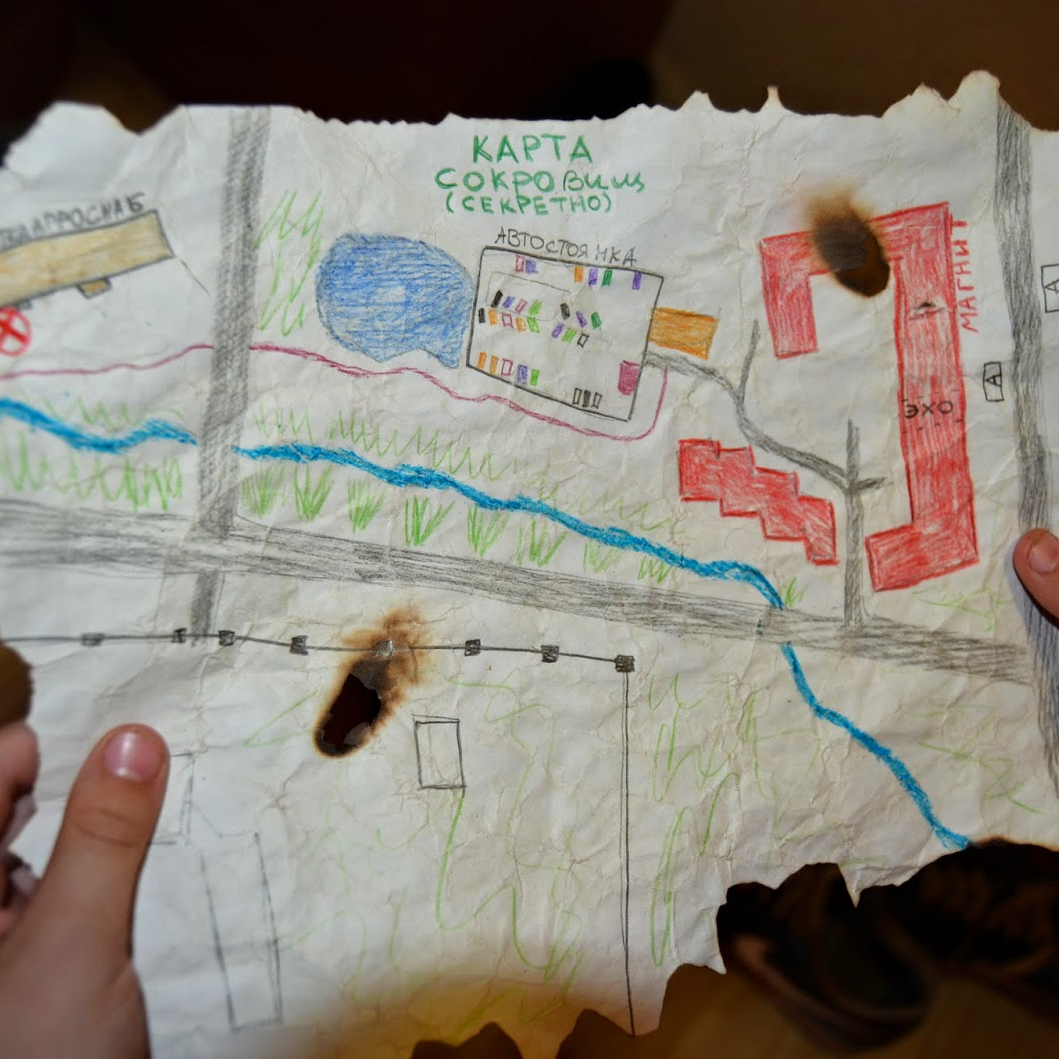
\includegraphics[scale=2]{map}}
    \caption{Карта сокровищ}
    \label{fig:image}
\end{figure}

\begin{lstlisting}[language=C++,caption=Код для поиска сокровищ]
    #include <stdio.h>
    
    int main(int) {
        printf("Hello world!");
        return 0;
    }
\end{lstlisting}

\hfill

В \verb|\LaTeX{}| можно создать ссылку почти на любой объект имеющий~номер --- на раздел, рисунок, формулу, пункт списка и~т.~п. При этом \verb|\LaTeX{}| сам позаботится о нумерации ссылок и ее обновлении по мере необходимости.

Команд для работы со ссылками всего три: \verb|\label|, \verb|\ref| и \verb|\pageref|, и они не зависят от того, на какой объект вы ссылаетесь.

С помощью \verb|\label{имя}| вы даете имя объекту, на который хотите сослаться --- помечаете его. В качестве примера создадим \verb|формулу|
\begin{verbatim}
\begin{equation}
ax^2+bx+c=0
\label{eq:sample}
\end{equation}
\end{verbatim}
и присвоим ей имя \verb|eq:sample|. В готовом документе это будет выглядеть так:
\begin{equation}
    ax^2+bx+c=0.
    \label{eq:sample}
\end{equation}

Чтобы сослаться на отмеченный объект используется команда\linebreak \verb|\ref{имя}|.
На ее месте в тексте документа будет напечатан номер, присвоенный объекту LaTeX'ом.
Так, поставив ссылку на указанную выше формулу мы увидим: (\ref{eq:sample}), хотя в исходном тексте документа стояло: \verb|\ref{eq:sample}|.

Наконец, команда \verb|\pageref{имя}| печатает номер страницы edf  сграницы, на которой расположен объект с данным именем.

Если вы сошлетесь на объект, имя которого не было предварительно задано командой \verb|\label|, LaTeX скомпилирует документ, но выдаст предупреждение:
\begin{verbatim}
LaTeX Warning: There were undefined references.
\end{verbatim}
и заменит команды \verb|\ref{неизвестное_имя}| на ''??'', так что неопределенную ссылку легко будет обнаружить.

Обработка документа, содержащего ссылки, происходит в два этапа: сначала компилятор сохраняет имена объектов (метки) и рассчитывает соответствующие им номера, затем он заменяет команды \verb|\ref| этими номерами. Поэтому документ со ссылками необходимо транслировать дважды. Если вы сделаете это только один раз, то LaTeX будет использовать информацию, которую он собрал во время предыдущей трансляции, и которая могла устареть. Однако LaTeX предупредит вас об этом:
\begin{verbatim}
LaTeX Warning: Label(s) may have changed. Rerun to get cross-references right.
\end{verbatim}
С помощью команды \verb|\pageref| вы можете указать читателю номер страницы, на которой находится интересующий его объект. Например, указав в файле \verb|.tex|:
\begin{verbatim}
См. формулу~(\ref{eq:sample}) на с.~\pageref{eq:sample}.
\end{verbatim}
получим в готовом документе:
\\[\baselineskip]
См. формулу~(\ref{eq:sample}) на с.~\pageref{eq:sample}.
\\[\baselineskip]
Поскольку одни и те же команды используются для ссылок на разные виды объектов, то в больших документах может возникнуть путаница, связанная с дублированием имен меток.

Допустим, мы хотим создать рисунок:
\begin{verbatim}
\begin{figure}[h]
\centering
Пример рисунка
\caption{Подпись}
\label{fig:sample}
\end{figure}
\end{verbatim}
\begin{figure}[h]
    \centering
    Пример рисунка
    \caption{Подпись}
    \label{fig:sample}
\end{figure}

Так как рисунок создан для примера, то использование метки \verb|sample| для него, как и для указанной выше формулы, выглядело бы логично. В результате возникло бы дублирование меток;
\begin{verbatim}
LaTeX Warning: Label 'sample' multiply defined.
\end{verbatim}

Мы избежали этой проблемы, добавив к метке префикс, указывающий на тип объекта. Префикс может быть произвольной строкой, но существуют общепринятые соглашения. Они перечислены в таблице.

\begin{table}[h]
    \centering
    \begin{tabular}{|l|l|l|}
        \hline
        Префикс: &     & Объект                            \\
        \hline
        chap:    &     & глава (chapter)                   \\
        \hline
        sec:     &     & раздел (section)                  \\
        \hline
        fig:     &     & рисунок (figure)                  \\
        \hline
        tab:     &     & таблица (table)                   \\
        \hline
        eq:      &     & уравнение (equation)              \\
        \hline
        lst:     &     & исходный код (listing)            \\
        \hline
        itm:     & xyz & пункт нумерованного списка (item) \\
        \hline
    \end{tabular}
\end{table}


Следуя им, обозначим ссылку на рисунок как\linebreak \verb|\label{fig:sample}|.

\hfill

\href{https://raw.githubusercontent.com/smartbyter/docstest/master/example.pdf}{Результирующий файл PDF}


\end{document}
